\documentclass[12pt, a4paper, oneside]{ctexart}
\usepackage{amsmath, amsthm, amssymb, bm, graphicx, hyperref, mathrsfs}

\title{\textbf{科研课堂课程作业}}
\author{黄伟宁}
\date{\today}
\linespread{1.5}
\newcounter{problemname}
\newenvironment{problem}{\stepcounter{problemname}\par\noindent\textbf{题目\arabic{problemname}. }}{\\\par}
\newenvironment{solution}{\par\noindent\textbf{解答. }}{\\\par}
\newenvironment{note}{\par\noindent\textbf{题目\arabic{problemname}的注记. }}{\\\par}
\usepackage{geometry}
\geometry{left=2.54cm,right=2.54cm,top=3.18cm,bottom=3.18cm}

\begin{document}

\maketitle
% \begin{problem}
% 这里是题目.
% \end{problem}

% \begin{solution}
%     这里是解答.
% \end{solution}

% \begin{note}
%     这里是注记.
% \end{note}

\begin{problem}
验证方程(1)通过变换(2)变换成方程(3):
\begin{gather}
    \frac{\partial \eta}{\partial t}=\frac{3}{2}\sqrt{\frac{g}{l}}\frac{\partial }{\partial x}(\frac{1}{2}\eta^{2} +\frac{2}{3}\alpha\eta+\frac{1}{3}\sigma\frac{\partial ^{2} \eta}{\partial  x^{2} }) \\
    t^{\prime}=\frac{1}{2}\sqrt{\frac{g}{l\sigma}}t,x^{\prime} = -\frac{x}{\sqrt{\sigma}},u=\frac{1}{2}\eta+\frac{1}{3}\alpha                                                                           \\
    \frac{\partial u}{\partial t}+6u\frac{\partial u}{\partial x}+\frac{\partial ^{3} u}{\partial x^{3} }=0.
\end{gather}
\end{problem}

\begin{solution}
    我们有
    $$
        \frac{\partial }{\partial t}=\frac{\partial }{\partial t^{\prime} }\frac{\mathrm{d}t^{\prime} }{\mathrm{d}t}=\frac{\partial }{\partial t^{\prime} }\cdot\frac{1}{2}\sqrt{\frac{g}{l\sigma}}
    $$
    $$
        \frac{\partial }{\partial x}=\frac{\partial }{\partial x^{\prime} }\frac{\mathrm{d}x^{\prime} }{\mathrm{d}x}=\frac{\partial }{\partial x^{\prime} }\cdot(-\frac{1}{\sqrt{\sigma}})
    $$
    $$
        \frac{\partial u }{\partial t}=\frac{1}{2}\frac{\partial \eta}{\partial t},\frac{\partial ^{2} u}{\partial x^{2} }=\frac{1}{2}\frac{\partial ^{2} \eta}{\partial x^{2} }
    $$

    代入之后有
    \begin{align*}
        \frac{\partial \eta}{\partial t} & =2\frac{\partial u}{\partial t}                                  \\
                                         & =\sqrt{\frac{g}{l\sigma}}\frac{\partial u}{\partial t^{\prime} }
    \end{align*}
    \begin{align*}
          & \frac{1}{2}\eta^{2} +\frac{2}{3}\alpha\eta+\frac{1}{3}\sigma\frac{\partial ^{2} \eta}{\partial x^{2} }                                   \\
        = & \frac{1}{2}(2u-\frac{2}{3}\alpha)^{2} +\frac{2}{3}\alpha(2u-\frac{2}{3}\alpha)+\frac{2}{3}\frac{\partial ^{2} u}{\partial x^{\prime 2} } \\
        = & 2u^{2} -\frac{2}{9}\alpha^{2} +\frac{2}{3}\frac{\partial ^{2} u}{\partial x^{\prime 2} }
    \end{align*}
    \begin{align*}
          & \frac{3}{2}\sqrt{\frac{g}{l}}\frac{\partial }{\partial x}(2u^{2} -\frac{2}{9}\alpha^{2} +\frac{2}{3}\frac{\partial ^{2} u}{\partial x^{\prime 2} }) \\
        = & -\frac{3}{2}\sqrt{\frac{g}{l\sigma}}(\frac{\partial (2u^{2} )}{\partial x^{\prime} }+\frac{2}{3}\frac{\partial ^{3} u}{\partial x^{\prime 3} })     \\
        = & -6\sqrt{\frac{g}{l\sigma}}u\frac{\partial u}{\partial x^{\prime} }-\sqrt{\frac{g}{l\sigma}}\frac{\partial ^{3} u}{\partial x^{\prime 3} }
    \end{align*}
    去掉“$ ^{\prime} $”标记之后,即可得到标准KdV方程:
    $$
        \frac{\partial u}{\partial t}+6u\frac{\partial u}{\partial x}+\frac{\partial ^{3} u}{\partial x^{3} }=0.
    $$
\end{solution}

\begin{problem}
验证KdV方程有行波解:
$$
    u(x,t)=\frac{c}{2}\text{sech}^{2} (\frac{\sqrt{c}}{2}(x-ct))
$$
\end{problem}

\begin{solution}
    计算可得
    \begin{gather*}
        \frac{\partial ^{3} u}{\partial x^{3} }=\frac{1}{2}c^{\frac{5}{2}} \text{tanh}(\frac{\sqrt{c}}{2}(x-ct))\text{sech}^2(\frac{\sqrt{c}}{2}(x-ct))(2\text{sech}^2(\frac{\sqrt{c}}{2}(x-ct))-\text{tanh}^2(\frac{\sqrt{c}}{2}(x-ct)))\\
        6u\frac{\partial u}{\partial x}=-\frac{3}{2}c^{\frac{5}{2}} \text{tanh}(\frac{\sqrt{c}}{2}(x-ct))\text{sech}^{4} (\frac{\sqrt{c}}{2}(x-ct))\\
        \frac{\partial u}{\partial t}=\frac{1}{2}c^{\frac{5}{2}}\text{tanh}(\frac{\sqrt{c}}{2}(x-ct))\text{sech}^{2} (\frac{\sqrt{c}}{2}(x-ct))
    \end{gather*}
    同时有
    $$
        \text{tanh}^{2} (x)=1-\text{sech}^{2} (x)
    $$
    代入即可验证行波解是KdV方程的解.
\end{solution}

\begin{problem}
画出行波解的图形
\end{problem}

\begin{solution}
    以下给出的为$ c=2 $ 时的图形
    \begin{figure}
        \centering
        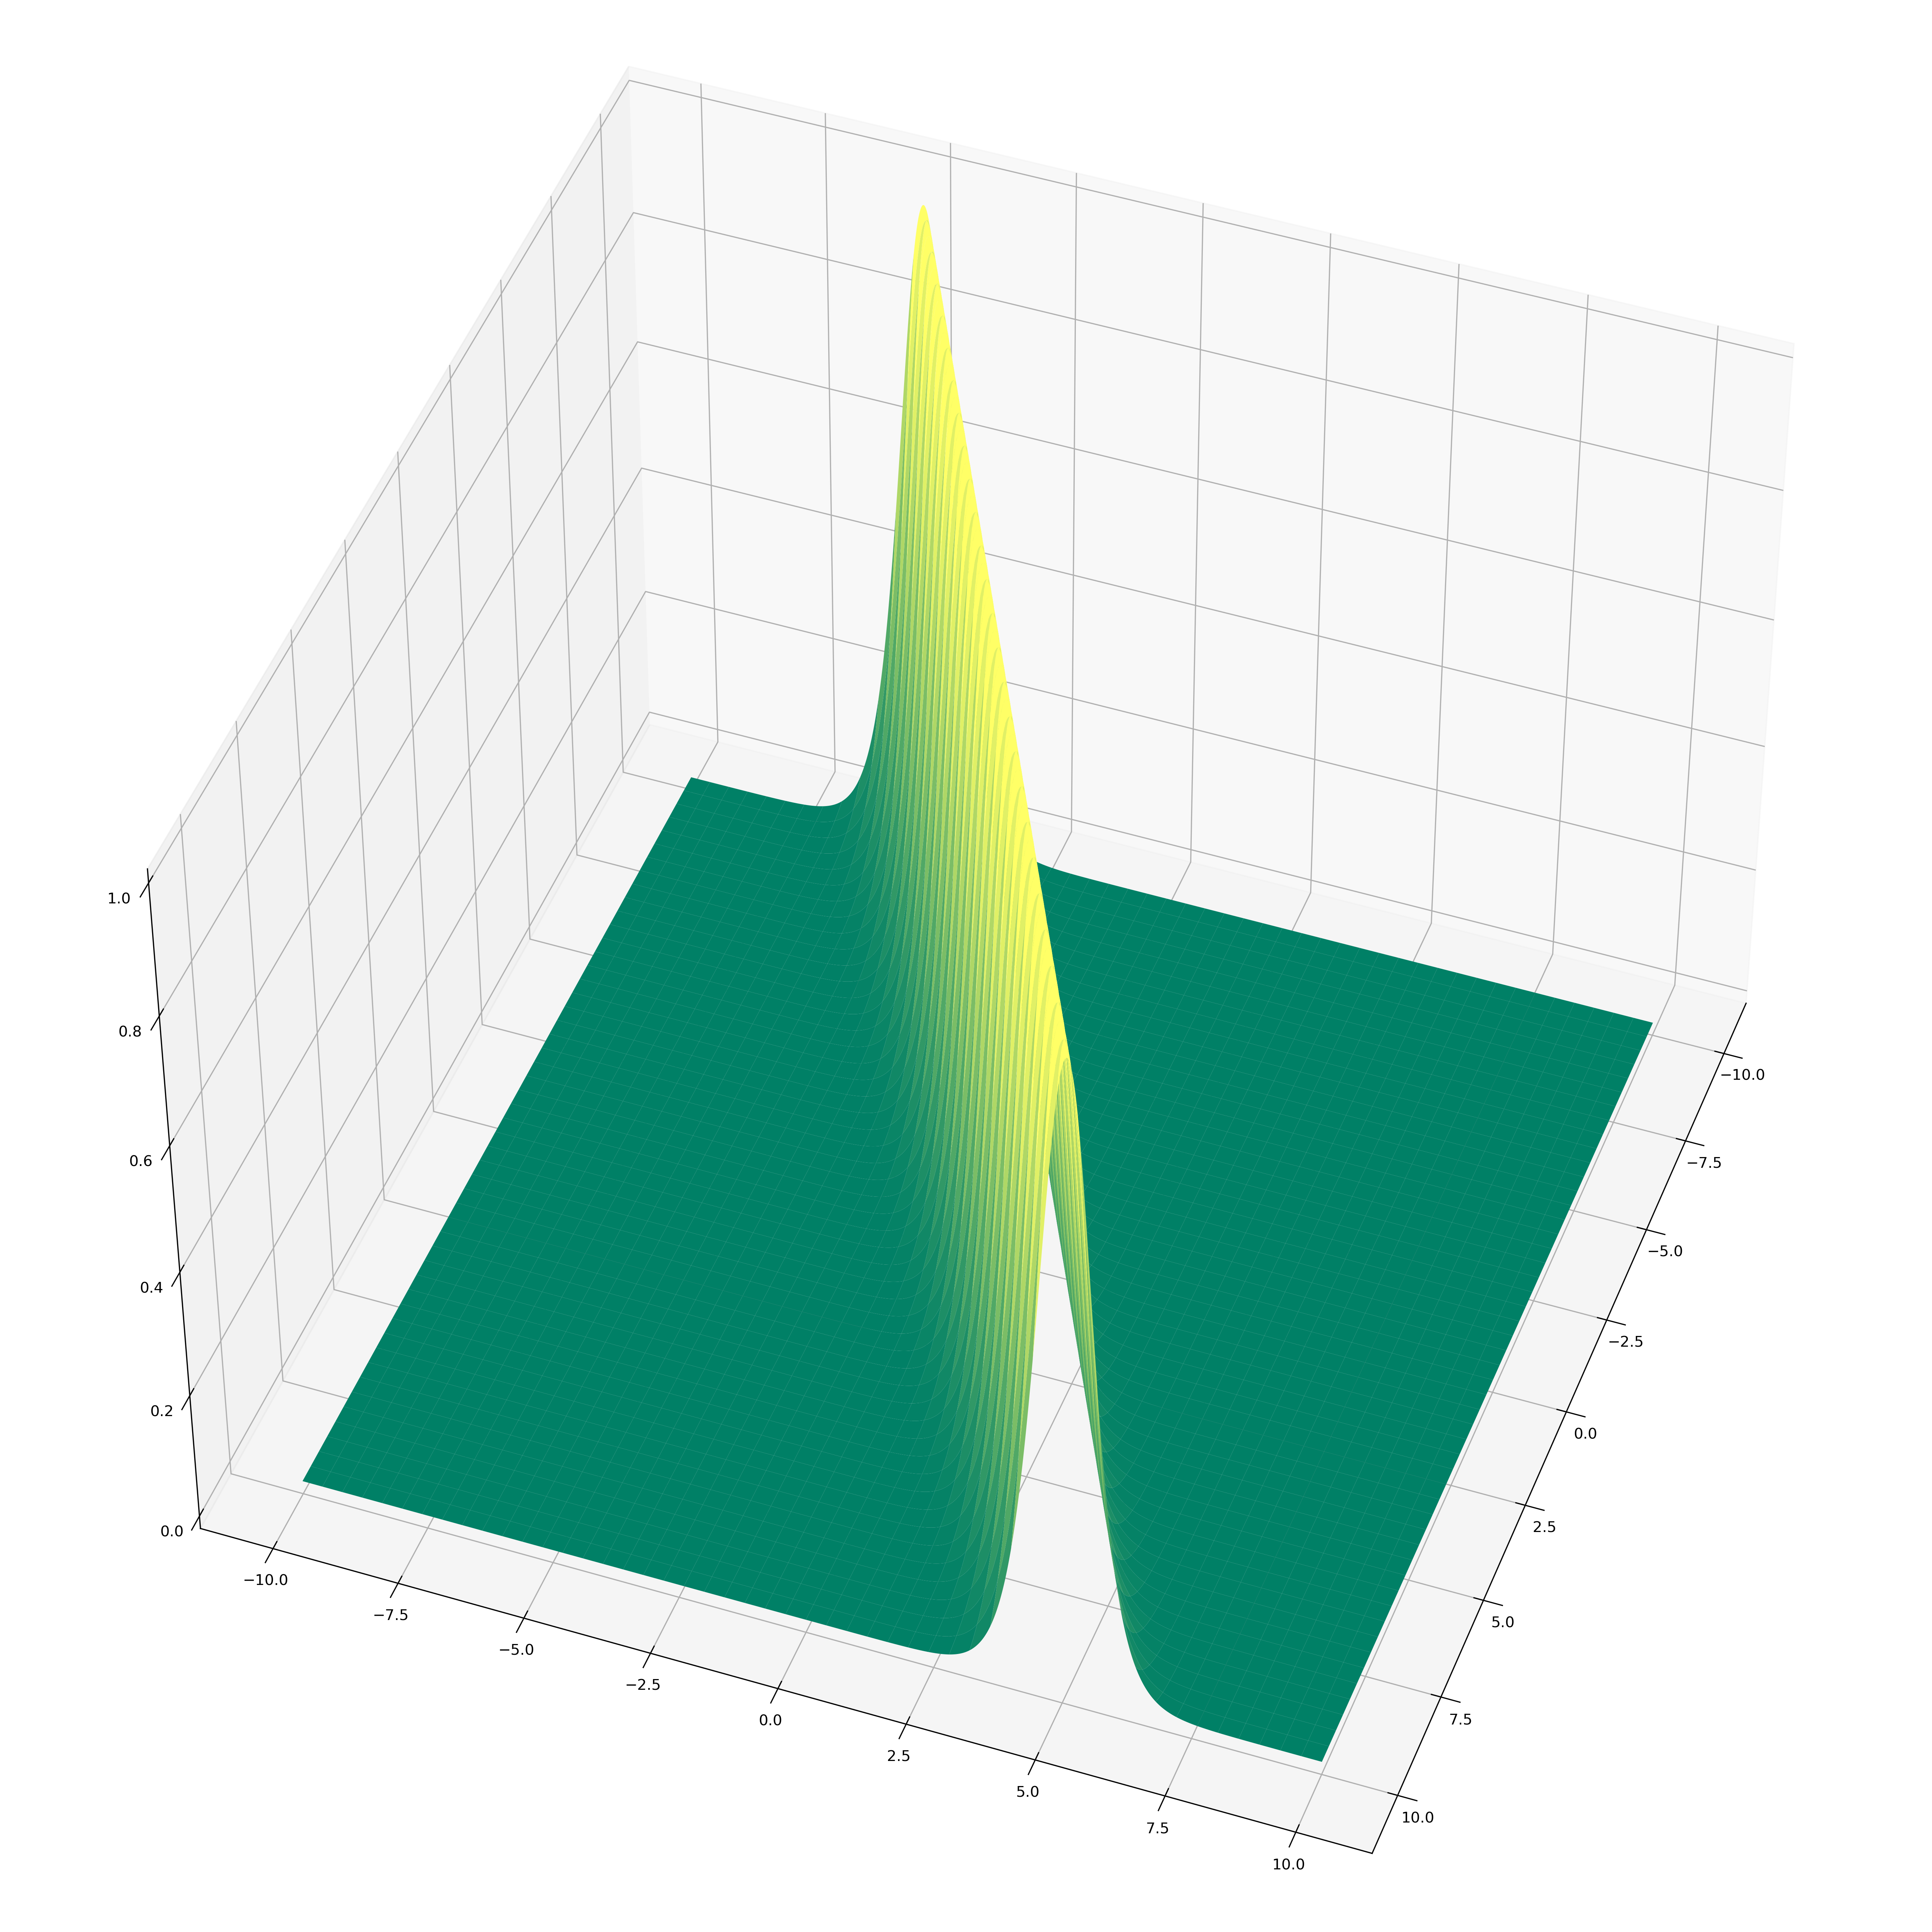
\includegraphics[scale=0.2]{picture/hw1.png}
        \caption{$ c=2 $ 时的行波解}
    \end{figure}
\end{solution}

\end{document}